The tool used in this work to achieve single-atom control is optical tweezers: by focussing a laser beam to a small enough spot it has been shown that under the right conditions, this trap can house at most one atom. 

\section{Loading Single Atoms}\label{sec:LoadingAtoms}

Single atom loading was first demonstrated by \cite{Schlosser2001}. 
Call the number of atoms in the tweezer $N$, \cite{Schlosser2002} suggested for the time-derivative of $N$ a model with contributions

\begin{equation}\label{LoadingTweezer}
	\frac{\text{d}N}{\text{d}t} = \alpha - \gamma N - \beta N(N-1)
\end{equation}

where the first term $\alpha$ is the loading rate or the amount of atoms entering the tweezer per second. 
Next, $\gamma$ is the atom loss as a result of collisions with the background gas. 
Lastly, $\gamma$ is a measure for the mainly 2 body loss as a result of light-assisted collisions.
3-body terms and higher are disregarded. 
In order to load single atoms, we must satisfy $\beta \gg \gamma$: the two-body collisions are dominant.
We can now look at two distinct scenarios:

\begin{itemize}
	\item Starting from 0 atoms in the tweezer: an additional atom entering will now load the tweezer to $N=1$. 
	
	\item Starting from $N=1$: when an additional atom is loaded, the atoms will immediately kick out each other because of the tiny tweezer volume and strong light intensity from the MOT beams. 
\end{itemize}

If the number of atoms at $t=0$ is larger than $N$, atoms will be lost in pairs until $N$ is either 0 or 1, after which the events above apply. 
Apparently, a loading event can lead to either 0 or 1 atom in the tweezer, both with $50\%$ probability. 
This is known as the collisional blockade effect. Experimentally demonstrated by \cite{Schlosser2001} and \cite{Schlosser2002} showed this effect to exits for 3 orders of magnitude in the loading rate $\alpha$.
Satisfying $\beta \gg \gamma$ can be done by keeping $\gamma$ to a minimum by going to the ultra high vacuum regime.
We intent to go to a pressure of the order of $10^{-10}$ mbar. In addition $\beta$ is maximized by going to high light-intensities and small trapping volumes. 
The remainder of this chapter is dedicated on how to minimize this trapping volume.

\section{Diffraction Limit}

The smallest achievable spot size is governed by the diffraction limit, which states that because light is a wave, it is impossible to focus down to an infinitely small spot even in the absence of aberrations.
Diffraction is elegantly described by Fourier optics \cite{Goodman2005}. 
We derive a result used throughout this work here.

\begin{mdframed}
    \subsection*{Intermezzo Fourier Optics}
    
    As we use the objective to make a tweezer, light is impinging on its back aperture. 
    We call its complex amplitude $U(x',y')$ and define the aperture at $z = 0$ on the optical axis.
    After the aperture, light will show diffraction. 
    An elegant description is provided by scalar diffraction theory.
    We will not repeat a full derivation here but we can refer the reader to \cite{Goodman2005}.
    Consider the Fresnel diffracion integral in cartesian coordinates. 
    After the aperture, the complex amplitude $U$ distribution is:
    
    \begin{equation}\label{eq:FresnelDiffraction}
        E(x,y,z) = 
        \frac{e^{ikz}}{i \lambda z} \iint_{-\infty}^{\infty} U(x',y',0) \exp{\frac{ik}{2z}} \exp{\left[(x-x')^2+(y-y')^2\right]} dx'dy'.
    \end{equation}
    
    In \cref{eq:FresnelDiffraction}, $\lambda$ is the wavelength, $k=2\pi/\lambda$ the wavenumber.
    In this thesis, we are usually not immediately interested in describing the light in the the near field of the aperture, but in the far-field. 
    More formally, the following needs to apply:
    
    \begin{equation}\label{eq:FraunhoferCriterion}
        z \gg k R^2/2,
    \end{equation}
    
    where $R$ is the maximum distance from the aperture to the optical axis. 
    While this criterion is in practice not met, it does hold in the focal point of a lens, because a lens projects an image in infinity to its focal length $f$. 
    Inserting \cref{eq:FraunhoferCriterion} in \cref{eq:FresnelDiffraction} yields:
    
    \begin{equation}\label{eq:FraunhoferDiffraction}
        E(x, y, z)=\frac{e^{i k z} e^{i k\left(x^{2}+y^{2}\right)/2}}{i \lambda z} \iint_{-\infty}^{\infty} U(x', y') \exp \left[\frac{-ik}{z}(x x'+y y')\right] dx' dy'
    \end{equation}. 
    
    This equation relates the field in the focus point point of the lens $U(x,y)$ to the field at the lens $U(x',y')$. 
    Contributins outside of the apeture can be discarded, and in practice we are not too intersted in the phase factor in front, such that we have
    
    \begin{equation}\label{eq:FraunhoferSimplified}
        E(x,y,z) \propto 
        \iint_{\text{aperture}} U(x',y') \exp{\left[- \frac{ik}{z}(xx'+yy')\right]}dx'dy'
    \end{equation}
    
    We recognize in \cref{eq:FraunhoferDiffraction} the spatial Fourier transform, in both $x$ and $y$ with respectively the frequencies $f_x = x/\lambda z$ and $f_y = y/\lambda z$, which is a result we will use later in this work. \cref{eq:FraunhoferDiffraction} is the Fraunhofer diffraction integral.
\end{mdframed}

 In this work, we are mostly concerned with circularly shaped apertures, for which a description in cylindrical coordinates is more natural.
 Ignoring the phase factor in front of the integral:

\begin{equation}\label{eq:FraunhoferRTheta}
    E(r,\theta, z) \propto \iint_{\text{aperture}} U(r') \exp{\left[
    -\frac{i k r r'}{z} \cos{(\theta-\theta')} 
    \right]}r'dr'd\theta'
\end{equation}

Using the integral definition of the Bessel function of the first kind\footnote{$J_0(x) = \frac{1}{2\pi} \int_0^{2\pi} \exp{(i x \cos{\alpha})} d\alpha$} we write \cref{eq:FraunhoferRTheta} as 

\begin{equation}\label{eq:FourierBessel}
    E(r,z) \propto 2\pi \int_0^{\infty} U(r') J_0\left( \frac{k r r'}{z}\right) r'dr'
\end{equation}

\cref{eq:FourierBessel} is the Fourier-Bessel or Hankel transform.
Now that the general formula has been derived, will make the problem more specific by introducing some parameters. 
In practice, we are interested in the focus point of the lens around $z \approx f$. 
We send a Gausian beam through the lens with an circular aperture function $U(r')$ with radius $R$, such that the input $E_i$ is

\begin{equation}\label{eq:GaussianAperture}
    E(r')=
    \begin{cases}
        e^{- w_i^2/R^2},& \text{if } r' < R\\
        0,               & \text{otherwise}
    \end{cases}
\end{equation}

Substituting \cref{eq:GaussianAperture} in \cref{eq:FourierBessel} yields

\begin{equation}\label{eq:FourierBesselAperture}
    E(r) \propto \int_0^R e^{-r'^2/w_i^2} J_0\left(\frac{k r r'}{f}\right)r'dr'
\end{equation}

\cref{eq:FourierBesselAperture} is analytically solvable for specific cases.
Letting $w_i/R$ go to infinity, which is to treat the incident Gaussian beam as a plane wave, we can neglect the exponential term in \cref{eq:FourierBesselAperture}. 
The integral is now tractable, yielding for the field amplitude

\begin{equation}\label{eq:AiryField}
    E(r) \propto \frac{f}{kRr} J_1\left(\frac{k R r}{f}\right)
\end{equation}

Taking the absolute value squared and normalizing yields the \ac{PSF}:

\begin{equation}\label{eq:NormalizedPSF}
    \frac{I}{I_0} = \left[
    \frac{2J_1(k r R/f)}{k r R/f}
    \right]^2
\end{equation}

\begin{figure}
    \centering
    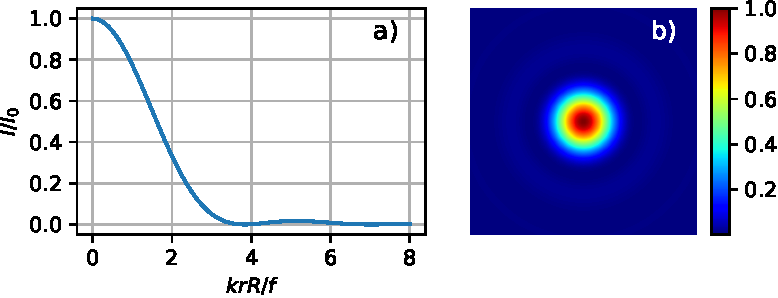
\includegraphics[width = 0.8\linewidth]{figures/AiryDisk.pdf}
    \caption{\textbf{a)} Normalized intensity of the perfect \ac{PSF} as a function of the azimuthal coordinate $r$ normalized in terms of units $f / kR$.
    \textbf{b) }2D plot of the Airy disk.  }
    \label{fig:AiryPlots}
\end{figure}

The point spread function of a circular aperture is shown in \cref{fig:AiryPlots}. 
Solving for the first zero of \cref{eq:NormalizedPSF}, and introducing the definition of numerical aperture for a compound microscope \ac{NA}: $R = \text{NA} \times f$ yields for this radius 

\begin{equation}\label{eq:Abbe}
    d_1 = 0.61 \frac{\lambdaup}{\text{NA}}
\end{equation}

This result is known as the Abbe limit or diffraction limit \cite{Abbe1882} and it is the smallest feature the imaging system can produce. 
To minimize the \ac{PSF} we can thus increase the \ac{NA} of our imaging system. In this work we will use $\text{NA} = 0.5$. 
For high NA imaging systems however, the paraxial approximation which was used to simplify the diffraction integral is no longer a priori true. 
Still, \cite{Chon2007} showed a derivation of \cref{eq:Abbe} using a different diffraction theory that does not require paraxial approximation and showed that for collimated laser beams \cref{eq:Abbe} has neglibible error even for $\text{NA} = 1$. 
We will assume we can still apply \cref{eq:Abbe} for $\text{NA} = 0.5$.

In practice, it is not convenient to use \cref{eq:FourierBesselAperture} to fit data and it is more convenient to use a simpler function. 
A Gaussian function is commonly used, and can even fit better than \cref{eq:FourierBesselAperture} because the rings of the Airy disk are easily deformed becauese of aberrations \cite{Knottnerus2018}. 

\mbox{}\par
\begin{mdframed}
    \subsection*{Intermezzo Gaussian Beams}\label{sec:GaussianBeams}
    
    Because we will frequenty use the parameters of a Gaussian beam, we will review them here. 
    Starting from Maxwell equations, one can derive under paraxial approximation a description of the transverse electromagnetic mode (TEM\textsubscript{00}) \cite{Leeuwen2017} for the electric field $E$.
    This Gaussian beam is most conveniently written down in cylindrical coordinates $\{r,z\}$:
    
    \begin{equation}\label{eq:GaussianBeam}
    	E(r,z) = \frac{w_0}{w(z)} \exp{\left(\frac{-r^2}{w^2(z)}\right)} \exp{\left[-ikz-i\frac{kr^2}{2R(z)} - i\psi(z)\right]},
    \end{equation}
    
    with parameters
    
    \begin{equation}\label{eq:GaussianBeamParameters}
    	k = \frac{2\pi}{\lambdaup}, \quad 
    	w(z) = \sqrt{w_0 + \frac{z^2}{z_R^2}}, \quad \text{and} \quad
    	R(z) = z \left(1 + \frac{z^2}{z_R^2}\right).
    \end{equation}
    
    Respectively, the wave number in terms of the wavelength $\lambdaup$, the beam waist, the radius where the field drops $1/e$ in terms of $w(z)\equiv w_0$ and $R(z)$ is the wavefront curvature. $z_R$ is the Rayleigh range, the distance along the optical axis where the beam waist has increased a factor of $\sqrt{2}$: $w(z=z_R) = \sqrt{2}w_0$.
    Finally $\psi(z)$ is an extra phase term originating from the curvature of the wavefront known as the Gouy phase.
    We find the intensity of the Gaussian beam by taking the absolute value squared:
    
    \begin{equation}\label{eq:GaussianBeamIntensity}
    	I(r,z) = I_0 \frac{w_0^2}{w^2(z)} \exp{\left(\frac{-2r^2}{w^2(z)}\right)}
    \end{equation}
    
    A sketch of a Gaussian beam profile is given in \cref{fig:GaussianBeam}, showing the $1/e$ field radius, or $1/e^2$ intensity radius $w_0$ and the Rayleigh range $z_R$. 
    
    \vspace*{3mm}
    \centering
        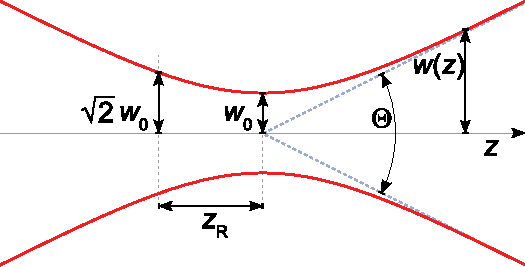
\includegraphics[width=0.5\linewidth]{figures/GaussianBeam.pdf}
        \captionof{figure}{Gaussian beam profile and some key parameters used in this work, the beam waist $w_0$ and Rayleigh range $z_R$. 
        Figure adapted from \cite{Hermans2009}.}
        \label{fig:GaussianBeam}
\end{mdframed}

Fitting this Gaussian as closesly as possible to an Airy pattern using a least-squares optimization, it can be shown that the equivalent Gaussian waist is \cite{Zhang2007}.

\begin{equation}\label{eq:GaussianAiryFit}
    w = 0.42 \frac{\lambdaup}{\text{NA}}
\end{equation}
 
If our measured waist is at this limit, the system is said to be diffraction limited, that is: the spot size is limited because of the wave character of light and not because of optical aberrations. 

\section{Optical Tweezers in Practice}\label{sec:TweezersPractice}

So to minimize the trapping volume, we need the highest possible numerical aperture. But there are more demands our lens should satisfy: the \ac{MOT} and subsequent \ac{ODT} are made in a vacuum chamber so the beam traverse a vacuum viewport. This poses additional requirements on the objective:

\begin{enumerate}
    \item Ultra-long working distance (the distance between the trap and the lens). For a single lens, this is equivalent to the focal length of course, though for a compound lens this is a bit more complicated. 
    
    \item Glass-thickness compensation. The relatively thick vacuum viewport will introduce significant (spherical) aberrations for high NA and therefore big angles. It is possible to correct for this by having an additional lens which will counteract this.
\end{enumerate}

To achieve this, we chose the G Plan Apo microscope objective from \textit{Mitutoyo}, as also used by \cite{Manuel2016,Ebadi2021}. 
This is an infinity-corrected objective, meaning light collected in its focussed is imaged at infinity (parallel beam) and an additional field lens is used to focus this image, such that the magnification is 

\begin{equation}\label{eq:InfinityMagnification}
    M = \frac{f_2}{f_1},
\end{equation}

where $f_2$ is the focal length of the field lens and $f_1$ the equivalent focal length of the objective\footnote{For a compound microscope objective, equivalent focal length means the focal length the objective would have when replaced by a single lens.}.
Relevant specifications of the objective are shown in \cref{table:MitutoyoSpecs}. 
From compound objectives, the equivalent focal length $f_1$ is defined in terms of the \ac{NA} and the back aperture radius of $R$ as $R = f_1 \text{NA} = 2$ mm. 

\begin{table}[h]
    \centering
    \caption{Key specifications of the objective from manufacterer Mitutoyo.}
    \label{table:MitutoyoSpecs}
    \begin{tabular}{l | l}
        \textbf{Specification}       & \textbf{Value} \\ \hline 
        NA                           & 0.5            \\ \hline
        Glass thickness compensation\footnote{We assume 3.5 mm of N-BK7 glass is used here, which has a slightly different refractive index than quartz for example.} & 3.5 mm         \\ \hline
        Equivalent focal length      & 4 mm           \\ \hline
        Working distance             & 15.08 mm      
    \end{tabular}
\end{table}

Because this objective was designed with visible wavelenghts in mind, it is probable that all of the lenses inside it are coated with a reflection coating that does not work well for the 800 nm regime. 
This is indeed the case, as we measured the tranmission of the objective to be just $(47 \pm 3)\%$ at 820 nm. We will therefore lose a significant of laser power. 
But this is not the only source of laser power loss: in producing the Airy pattern we assumed plane wave illumination, but in practice laser beams have Gausian shape. 
As a result, when working with a beam significantly larger than the back aperture this excess power is lost. 
Assuming the beam is aligned with the center of the aperture, the power tranmission $P/P_0$ as a function of the incident waist $w_i$ is

\begin{equation}\label{eq:fracPowerCircular}
    P/P_0 = 1 - e^{-2w_i^2/R^2}
\end{equation}

which tends to zero for very wide beams (plane waves). Clearly there is an optimum sommewhere.
To illustrate this, we will look at the other extreme case of $w_i \ll R$. 
The waist is much smaller than the aperture, according to \cref{eq:fracPowerCircular} all of the power is transmitted through the aperture.
We let the integration boundary run to infinity and using a Hankel tranform pair\footnote{$F_0(k) = \int_0^{\infty} e^{-1/2 a^2 r^2} J_0(k r)r dr = \frac{1}{a^2} e^{-\frac{k^2}{2a^2}}$} find 

\begin{equation}\label{eq:GaussianCase}
    U(r) \propto \frac{w_i^2}{2} \exp{\left(\frac{-k^2w_i^2 r^2}{2f^2}\right)}.
\end{equation}

The result is a Gaussian, but with a modified waist of $\lambdaup f / \pi w_0$.
This modified waist will go up for smaller $w_0$ (Fourier transform property). 
Clearly, this is not ideal either. 
To understand the optimum a bit better, we will define the concept of trap frequencies. 
But a priori we know the resulting potential will be something in between a Gaussian beam and an Airy pattern. 

\subsection{Tweezer Potential}

From \cref{eq:Stark} we know that the potential of the tweezer is proportional to the light intensity. 
Assuming a Gaussian tweezer beam, the potential $U$ in cylindrical coordinates will be roughly (\cref{eq:GaussianBeam,eq:GaussianBeamParameters}).

\begin{equation}\label{eq:GaussianPotential}
    U(r,z)=\frac{-U_{0}}{1+z^{2} / z_{R}^{2}} \exp \left(\frac{-2 r^{2}}{w_{0}^{2}\left(1+z^{2} / z_{R}^{2}\right)}\right)
\end{equation}

\cref{eq:GaussianPotential} is plotted in \cref{fig:GaussianPotential} for normalized radial coordinate $r/w_0$ as well as longitudinal coordinate $z_R$. 
This is not to scale: the Rayleigh range $z_R$ is typically bigger than the waist $w_0$.
Assuming a Gaussian is justified because near the center, an Airy disk and Gaussian beam are nearly identical.
We are interested in potentials much deeper than the temperature of the atoms, such that the atoms will mostly occupy the bottom of the tweezer. 
Taylor expanding \cref{eq:GaussianPotential} around $(r,z)=(0,0)$ to second order yields 

\begin{figure}
    \centering
    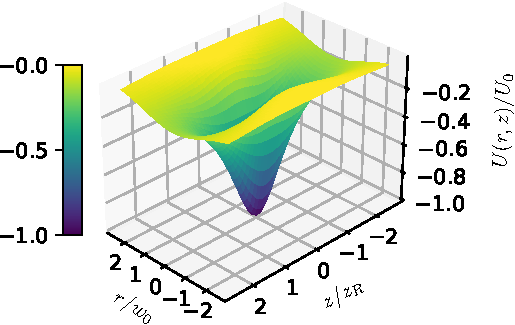
\includegraphics[width=.56\linewidth]{figures/GaussianPotential.pdf}
    \caption{Normalized potential from a Gaussian intensity shape. The independent coordinates are the normalized cylindrical coordiantes $r/w_0$ and $z/z_R$.}
    \label{fig:GaussianPotential}
\end{figure}

\begin{equation}\label{eq:ApproximateGaussianPotential}
    U(r,z) \sim -U_0 - 2U_0 \frac{r^2}{w_0^2} - 2U_0 \frac{z^2}{z_R^2}
\end{equation}

For this harmonic potential, one can compute the harmonic oscillation frequencies 

\begin{equation}\label{eq:TrapFrequencies}
    \omega_r = 2\left(\frac{U_0}{m w_0^2}\right)^{1/2}, \quad
    \omega_z= \left(\frac{2 U_0}{m z_R^2}\right)^{1/2}
\end{equation}

Because $z_R > w_0$, the longitudinal oscillation frequency is lower than the radial frequency. 
Trap frequencies are a nice property to optimize, because from the definition, higher trap frequencies translate to deeper as well as sharper tweezers. 
\cite{Madjarov2021} optimized \cref{eq:TrapFrequencies} for the $w_i/R$ ratio and found an optimum around $w_i\sim R$, which we will use in this work\footnote{Because trap frequencies can be probed exprimentally, they can be used to perform post-corrections on tweezer arrays as well as shown by \cite{Ebadi2021}.}.

\section{Measuring the Tweezer potential}

We would like to measure tweezer potential made by our microscope objective. 
We could use time symmetry and look at the reverse direction: using the objective to look at a pinhole, retrieving its \acf{PSF} \cite{Knottnerus2018,Sortais2007}
However, using this method the objective will produce a plane wave, when we know that in practice we do not send a plane wave to the objective as discussed in \cref{sec:TweezersPractice}
function. 

Instead, we used another microscope objective, to look into produced tweezer potential by the \textit{Mitutoyo}. 
In doing this, the tweezer potential will be convolved with the \ac{PSF} of the second microscope objective\cite{Baumgaertner2017}.
Therefore we used a second microscope objective\footnote{Newport M-60X 0.85 NA objective.} with significantly higher \ac{NA}, minimizing this effect. 

\subsection{Optical Setup}

In the actual machine, we use an optically contacted glass cell as our vacuum chamber. Because no objective exists that has significantly higher NA than 0.5 as well as ultra-long working distance, we can not look into the glass cell using this method. Therefore, we use a piece of glass with the same thickness and material (quartz glass, $d = 4.0$) mm to imitate the glass cell. The second objective will produce an image onto a linear CCD camera\footnote{Point Grey FLEA2 FL2-08S2M.}. Because alignment of the Mitutoyo objective with the incident beam, as well as alignment of the two objectives with respect to each other is crucial, both objectives are mounted on piezo-controlled 5 axis translation stages. 
This is drawn in the lower-right corner of \cref{fig:TiSandSLMsetup}.

On top we show the laser source used.
This laser is positioned on a separate table and its output is brought to the main table using a \ac{PM} optical fiber. 
The laser source is a \ac{Ti:S} ring laser\footnote{\textit{Coherent} 899-21 ring laser} (linewidth $\sim 1$ Mhz, output power max. $\sim 1$ W.). 
The crystal is pumped using a pump laser\footnote{\textit{Coherent} Verdi V18} (18W power, 532 nm). 
The \ac{Ti:S} is eaily tunable in wavelength over a wide range. For Sr 813 will be used, but for the experiments for Rb we used 820 nm. 
In between the laser source and the objective, there is a \ac{SLM}. But the SLM has its own \cref{ch:arrays}, so will not get into that now. 
In day to day tuning of the mirrors inside the Ti:S ring laser, the output angle and therefore the fiber coupling efficiency is slightly changed. 
To ease the coupling, we run a coax cable from a power meter on the main table to a multimeter on the Ti:S table. 

\begin{figure}
    \centering
    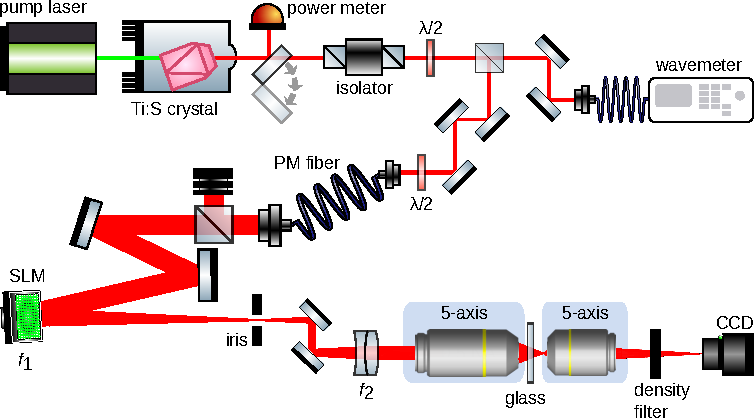
\includegraphics[width=0.8\linewidth]{figures/TiSandSLM.pdf}
    \caption{Optical setup for making an optical tweezer and imaging this tweezer onto a CCD camera. 
    Laser source decribed int the text and \ac{SLM} more thoroughly in \cref{ch:arrays}.
    The titanium sapphire laser is positioned on a separate table. 
    All cubes are polarizing.}
    \label{fig:TiSandSLMsetup}
\end{figure}

\subsection{Calibration Imaging System}

\begin{figure}
    \centering
    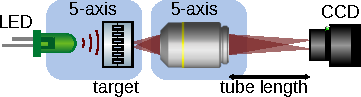
\includegraphics[width = 0.5\linewidth]{figures/LEDcalibration.pdf}
    \caption{Illumination of the calibration target by an LED, imaged by the 0.85 NA objective and camera at fixed distance.}
    \label{fig:resolutionTarget}
\end{figure}

The 60X magnification of the 0.85 NA objective is only specified when used in a microscope with standard tube length distance, because it is finite conjugate corrected.
Outside of a standard microscope, we have to calibrate its exact magnification.
We do this using a high resolution target\footnote{Technologie Manufaktur TC-RT01}, featuring groups of lines with variable spacing between them. 
The way this was done is shown in \cref{fig:resolutionTarget}.
Initially, we tried to use laser light to illuminate the target, but we did not get a clear image. 
Most likely this is because of the diffracting beams interfering with each other. 
To combat this we used light from an incoherent light source (\ac{LED}). We neglect the slightly different focus point from the Newport objective for our laser frequency compared to white light. 

\begin{figure}
    \centering
    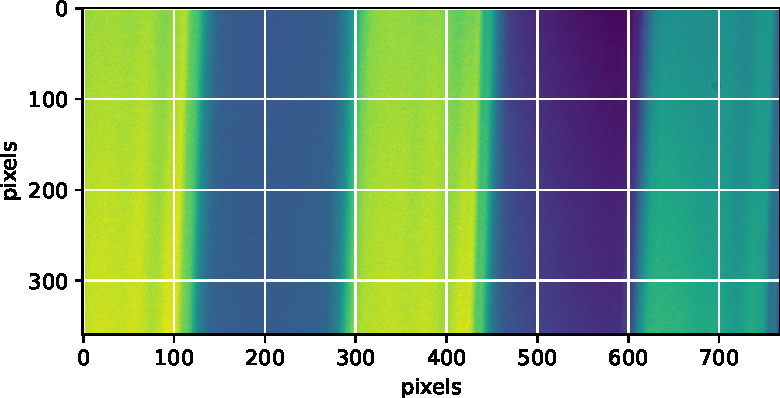
\includegraphics[width = 0.42\linewidth]{figures/LineSpacingCalibration.pdf}
    \caption{Image from the resolution target illuminated showing lines spaced by 45 lines per mm.}
    \label{fig:resolutionTarget}
\end{figure}

To detect the edges in \cref{fig:resolutionTarget}, we use an edge detection algorithm script.
For several 1D row slices of the image, it blurs the edge using a Gaussian to suppress noise and subsequently computes the spatial derivative. 
When the derivative surpasses a set threshold we define it as an edge.
Dividing the pixel spacing of the lines by the pixel pitch of the camera ($4.65$ $\mu$m) we find a magnification of ($67 \pm 3$)X, which is larger than the 60X specified by Newport. 
We attribute this to a slightly longer objective-camera distance that was used. 
After the calibration was performed, the objective-camera distance was left untouched. 

\section{Tweezer Images: Radial}

An image of the CCD camera is shown in \cref{fig:SingleSpotZoomed}. 
There seems to be a small tilt aberration present as the side ring is more clearly visible on the right side. 
We found aberrations of this magnitude almost impossible to get rid of, as it could originate from anywhere between the input beam and the camera.

In \cref{fig:AzimuthalAverage} we have integrated the intensity in rings around the maximum with a width of 1 pixel, effectively computing an azimuthal average. 
This result is compared against the \ac{PSF} of the objective (\cref{eq:NormalizedPSF}), as well as the result from scalar diffraction theory using a Gaussian input beam equal to the aperture $w_i \sim R$, which was obtained by computing \cref{eq:FourierBesselAperture} for a sample of radial coordinates $r$. 

\begin{figure}
    \centering
    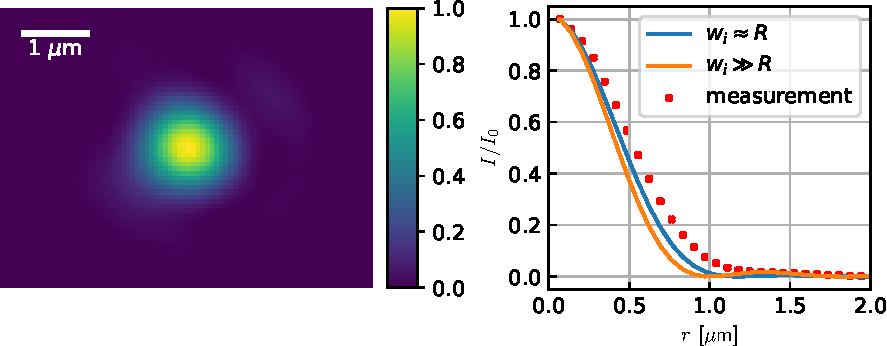
\includegraphics[width=\linewidth]{figures/AzimuthalAverageSpotZoomed.pdf}
    \caption{\textbf{a)} Tweezer as imaged by the second objective onto the CCD camera. 
	\textbf{ b)} Azimuthal average (red) plotted against the \ac{PSF}, \cref{eq:NormalizedPSF} of the objective as well as the Gaussian input beam formula \cref{eq:FourierBesselAperture}.}
    \label{fig:2Dresults}
\end{figure}


So, if a Gaussian input beam used, the resulting spot will be slightly broader.
Additionally, the rings of the Airy disk will be slightly surpressed, this effect is known as Gaussian apodization.
This plot is convenient for showing the general behavior, but is not accurate enough to extract data like the waist. 
For example: in this binning method, distance to the center pixel are calculated, but the center could be anywhere on this pixel. 
Therefore we also perform a two-dimensional Gaussian fit using \cref{eq:2DGaussian}.

\begin{equation}\label{eq:2DGaussian}
    \frac{G(x,y)}{G_0} =  
    \exp{\left[ -\frac{(x-x_0)^2}{2\sigma_x^2}\right]}
    \exp{\left[ -\frac{(y-x_0)^2}{2\sigma_y^2}\right]}
\end{equation}

The result of this fit is shown in \cref{fig:3Dshowing}. 
Cleary, the obtained tweezer potential fits very well to a Gaussian, which justifies the assumption of using a Gaussian approximation to estimate the trap frequencies (\cref{eq:GaussianPotential}. 
This is confirmed by the coefficient of determination $R^2 > 0.99$.

\begin{figure}
\centering
	\begin{subfigure}{.49\textwidth}
	    \centering
		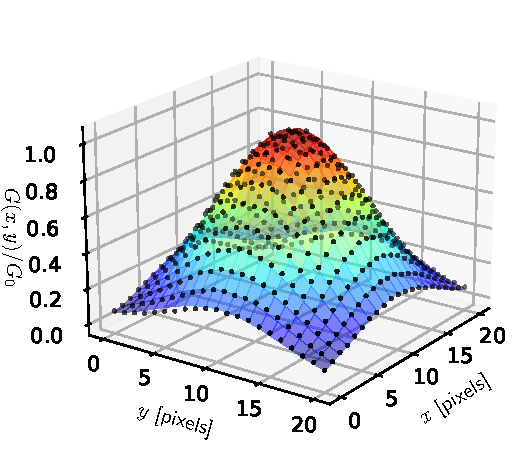
\includegraphics[width=0.96\linewidth]{figures/3DSpotFitGaussian.pdf}
		\caption{}
		\label{fig:3Dshowing}
	\end{subfigure}
	\begin{subfigure}{.49\textwidth}
		\centering
		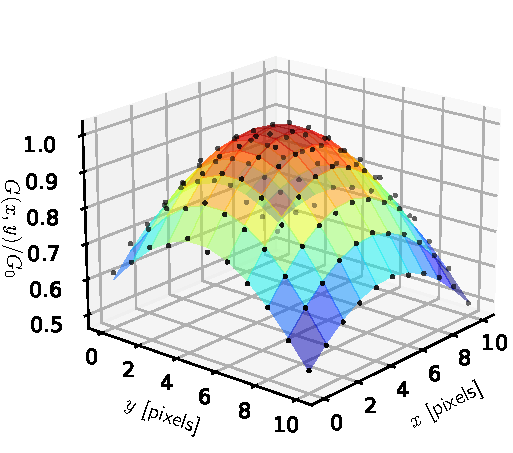
\includegraphics[width=0.96\linewidth]{figures/3DSpotFitGaussianSmaller.pdf}
		\caption{}
		\label{fig:3Dwaistfit}
	\end{subfigure}
	\caption{\textbf{a)} Plot showing convergence of the Gaussian fit. $R^2 > 0.99$.
	\textbf{ b)} Region of interest around the maximum that was used to extract the waist.}
	\label{fig:3Dfits}
\end{figure}

Assuming the $\sigma_x \sim \sigma_y$ which should be the case for a circlar aperture, we find the waist as $w_0 = \sigma_x + \sigma_y = (0.88 \pm 0.04)$ $\mu$m, where the error originates mainly from the calibration of the magnification. 
In order to find this waist, a smaller, 10 by 10 pixel region of interest was used, see \cref{fig:3Dfits}.
Despite the 0.85 NA used, there will still be a slight convolution with the imaging point spread function present. 
Although in deconvolution is non-trivial in general, for a Gaussian it is quite straightforward \cite{Knottnerus2018} in terms of the waists of the image and the diffraction-limited waist of the imaging system:

\begin{equation}\label{eq:Deconvolution}
    w_{\text{object}} = \sqrt{w_{\text{image}}^2-w_{\text{system}}^2}.
\end{equation}

This gives an object waist of $w_{\text{obj}} = (0.77 \pm 0.05)$ $\mu$m. 
Comparing to the theory result, for $\lambdaup = 820$ nm and $\text{NA} = 0.5$ (\cref{eq:Abbe,eq:GaussianAiryFit}) yields $w_0 = 0.689$ $\mu$m. 
But this result unachievale because of $w_i \sim R$ used. 
We know that as a result of this, the waist should be $\approx$9-10\% larger \cite{Sortais2007,Chon2007} which was confirmed by \cref{eq:FourierBesselAperture}, yielding $w_0 \sim 0.75$ $\mu$m, which lies within the error margin.
We conclude the tweezer is nearly diffraction-limited in size.

We did apply some aberration correction, which is mainly described in the next section \cref{sec:Tweezer3D}.
The result shown is after this aberration correction, though this this not significantly improve the result. 
We did note an improvement mainly for the axial direction which the next section is about. 


\section{Tweezer: Axial Direction}\label{sec:Tweezer3D}

For the volume of the tweezer not only the radial direction is important, but the axial (longitudinal) direction as well. 
The relevevant quantity here is the Rayleigh range (see \cref{fig:GaussianBeam}).
For the radial images shown in \cref{fig:2Dresults} we were intially surprised that the results was already pretty good even before aberration correction, because we know for example that the optical thickness of the glass cell (and the quartz plate that replaces the glass cell, \cref{fig:TiSandSLMsetup} is about 0.5 mm too thick: the objective is designed for 3.5 mm of N-BK7 (refractive inded $n = 1.51$, $nd = 5.3$ mm) whereas the cell is 4.0 mm of quartz glass ($n = 1.44$, $nd = 5.8$ mm). 
This might seem insignicant, but because of the high \ac{NA} and consequently large angles under which the light traverses the glass, it is possible the outer (marginal) rays will focus at at a slightly different point than the inner (paraxial) rays. 
To study the axial direction, we scan the Mitutoyo objective along the optical ($z$) axis and record an image of the tweezer. 
In the end, all images are stiched together to make a single image that would give an idea of a sideview of the tweezer.
To calibrate the amount of translation we calibrated the step size of the motor. The optical setup is shown in \cref{fig:ZScanSetup}

\begin{figure}
    \centering
    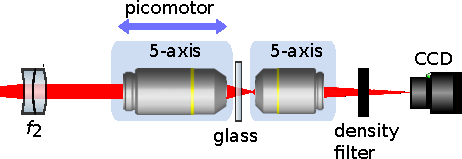
\includegraphics[width=0.6\linewidth]{figures/ZScanSetup.pdf}
    \caption{Optical setup}
    \label{fig:ZScanSetup}
\end{figure}

\begin{figure}
\centering
	\begin{subfigure}{.49\textwidth}
	    \centering
		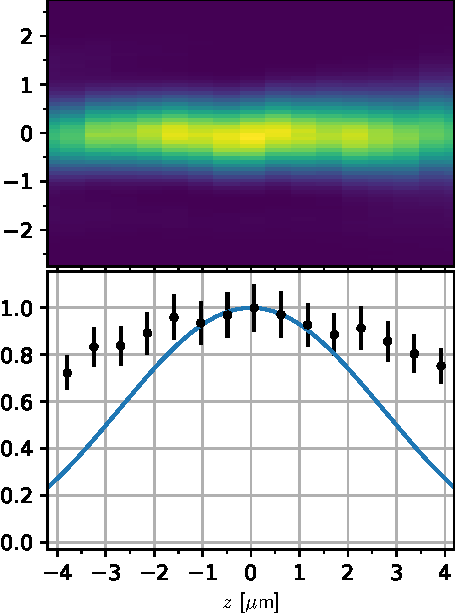
\includegraphics[height=9.5cm]{figures/AxialImageTweezerScanUncorrected.pdf}
		\caption{}
		\label{fig:AxialUncorrected}
	\end{subfigure}
	\begin{subfigure}{.49\textwidth}
		\centering
		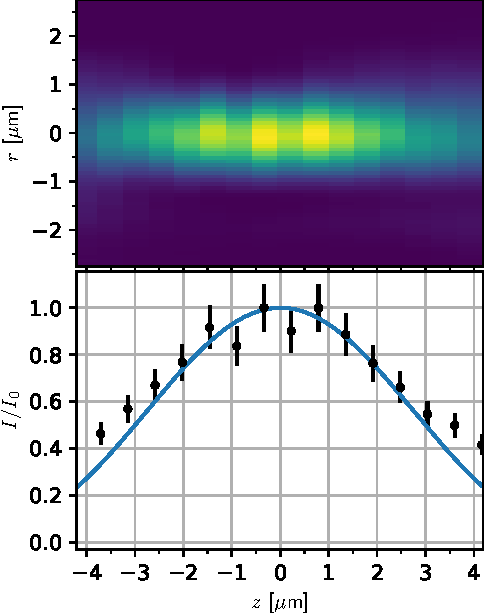
\includegraphics[height=9.5cm]{figures/AxialImageTweezerScan.pdf}
		\caption{}
		\label{fig:AxialZernike}
	\end{subfigure}
	\caption{Radial intensity profile \textbf{a)} before aberration correction: $z_R \sim 6.2$ $\mu$m and \textbf{b)} after aberration correction: $z_R \sim 3.5$ $\mu$m.}
	\label{fig:AxialScans}
\end{figure}


\subsection{Picomotor Attenuator Calibration}

Piezo-controlled attenuaters are very good at producing minisclule ($<30$ mm) step sizes. The step size is also extremely constant, making them ideal for axials scans like this.
The stage we used is 8081-M 5-axis motorized tilt aligner from Newport. 
Because of the 5 degrees of freedom, it can accurately align the two objectives with each other. 
To drive this stage, we used a set of Newport 8742 controllers in daisy-chain configuration: both can drive 4 motors so we have 2 of them to address all 5 motors.
For scanning the axial direction of the tweezer we only use one of the 5 motors inthe stage. 
However, to know the exact step size calibration is needed because the step size is dependent on the torque applied, which depends on the direction of travel as well as whether the motor has to counter gravity, etc.
In order to do this, we repeatedly measured the available translation range of some $\sim$ 3mm, recording the amount of steps this takes as well as the amount moved using a caliper. 
We found a step calibration of $10.6 \pm 0.2$ $\mu$m/step, which was used to translate amount of steps to distances. 

\section{Tweezer Images: Axial}

In \cref{fig:AxialUncorrected} the scanned profile of the tweezer is shown . 
Also plotted is the result from Fraunhofer diffraction theory.











